\documentclass[twoside]{book}

% Packages required by doxygen
\usepackage{fixltx2e}
\usepackage{calc}
\usepackage{doxygen}
\usepackage[export]{adjustbox} % also loads graphicx
\usepackage{graphicx}
\usepackage[utf8]{inputenc}
\usepackage{makeidx}
\usepackage{multicol}
\usepackage{multirow}
\PassOptionsToPackage{warn}{textcomp}
\usepackage{textcomp}
\usepackage[nointegrals]{wasysym}
\usepackage[table]{xcolor}

% Font selection
\usepackage[T1]{fontenc}
\usepackage[scaled=.90]{helvet}
\usepackage{courier}
\usepackage{amssymb}
\usepackage{sectsty}
\renewcommand{\familydefault}{\sfdefault}
\allsectionsfont{%
  \fontseries{bc}\selectfont%
  \color{darkgray}%
}
\renewcommand{\DoxyLabelFont}{%
  \fontseries{bc}\selectfont%
  \color{darkgray}%
}
\newcommand{\+}{\discretionary{\mbox{\scriptsize$\hookleftarrow$}}{}{}}

% Page & text layout
\usepackage{geometry}
\geometry{%
  a4paper,%
  top=2.5cm,%
  bottom=2.5cm,%
  left=2.5cm,%
  right=2.5cm%
}
\tolerance=750
\hfuzz=15pt
\hbadness=750
\setlength{\emergencystretch}{15pt}
\setlength{\parindent}{0cm}
\setlength{\parskip}{3ex plus 2ex minus 2ex}
\makeatletter
\renewcommand{\paragraph}{%
  \@startsection{paragraph}{4}{0ex}{-1.0ex}{1.0ex}{%
    \normalfont\normalsize\bfseries\SS@parafont%
  }%
}
\renewcommand{\subparagraph}{%
  \@startsection{subparagraph}{5}{0ex}{-1.0ex}{1.0ex}{%
    \normalfont\normalsize\bfseries\SS@subparafont%
  }%
}
\makeatother

% Headers & footers
\usepackage{fancyhdr}
\pagestyle{fancyplain}
\fancyhead[LE]{\fancyplain{}{\bfseries\thepage}}
\fancyhead[CE]{\fancyplain{}{}}
\fancyhead[RE]{\fancyplain{}{\bfseries\leftmark}}
\fancyhead[LO]{\fancyplain{}{\bfseries\rightmark}}
\fancyhead[CO]{\fancyplain{}{}}
\fancyhead[RO]{\fancyplain{}{\bfseries\thepage}}
\fancyfoot[LE]{\fancyplain{}{}}
\fancyfoot[CE]{\fancyplain{}{}}
\fancyfoot[RE]{\fancyplain{}{\bfseries\scriptsize Generated by Doxygen }}
\fancyfoot[LO]{\fancyplain{}{\bfseries\scriptsize Generated by Doxygen }}
\fancyfoot[CO]{\fancyplain{}{}}
\fancyfoot[RO]{\fancyplain{}{}}
\renewcommand{\footrulewidth}{0.4pt}
\renewcommand{\chaptermark}[1]{%
  \markboth{#1}{}%
}
\renewcommand{\sectionmark}[1]{%
  \markright{\thesection\ #1}%
}

% Indices & bibliography
\usepackage{natbib}
\usepackage[titles]{tocloft}
\setcounter{tocdepth}{3}
\setcounter{secnumdepth}{5}
\makeindex

% Hyperlinks (required, but should be loaded last)
\usepackage{ifpdf}
\ifpdf
  \usepackage[pdftex,pagebackref=true]{hyperref}
\else
  \usepackage[ps2pdf,pagebackref=true]{hyperref}
\fi
\hypersetup{%
  colorlinks=true,%
  linkcolor=blue,%
  citecolor=blue,%
  unicode%
}

% Custom commands
\newcommand{\clearemptydoublepage}{%
  \newpage{\pagestyle{empty}\cleardoublepage}%
}

\usepackage{caption}
\captionsetup{labelsep=space,justification=centering,font={bf},singlelinecheck=off,skip=4pt,position=top}

%===== C O N T E N T S =====

\begin{document}

% Titlepage & ToC
\hypersetup{pageanchor=false,
             bookmarksnumbered=true,
             pdfencoding=unicode
            }
\pagenumbering{alph}
\begin{titlepage}
\vspace*{7cm}
\begin{center}%
{\Large mpm \\[1ex]\large Alpha }\\
\vspace*{1cm}
{\large Generated by Doxygen 1.8.13}\\
\end{center}
\end{titlepage}
\clearemptydoublepage
\pagenumbering{roman}
\tableofcontents
\clearemptydoublepage
\pagenumbering{arabic}
\hypersetup{pageanchor=true}

%--- Begin generated contents ---
\chapter{Namespace Index}
\section{Namespace List}
Here is a list of all documented namespaces with brief descriptions\+:\begin{DoxyCompactList}
\item\contentsline{section}{\hyperlink{namespacemfm}{mfm} \\*\hyperlink{classmfm_1_1_m_f_m}{M\+FM} namespace }{\pageref{namespacemfm}}{}
\end{DoxyCompactList}

\chapter{Hierarchical Index}
\section{Class Hierarchy}
This inheritance list is sorted roughly, but not completely, alphabetically\+:\begin{DoxyCompactList}
\item \contentsline{section}{mfm\+:\+:Blockset$<$ Tdim $>$}{\pageref{classmfm_1_1_blockset}}{}
\item \contentsline{section}{mfm\+:\+:Domain$<$ Tdim $>$}{\pageref{classmfm_1_1_domain}}{}
\item \contentsline{section}{mfm\+:\+:Element$<$ dim $>$}{\pageref{classmfm_1_1_element}}{}
\item \contentsline{section}{mfm\+:\+:IO}{\pageref{classmfm_1_1_i_o}}{}
\item \contentsline{section}{mfm\+:\+:Material$<$ dim $>$}{\pageref{classmfm_1_1_material}}{}
\item \contentsline{section}{Material\+Point$<$ Tdim $>$}{\pageref{class_material_point}}{}
\item \contentsline{section}{mfm\+:\+:M\+FM}{\pageref{classmfm_1_1_m_f_m}}{}
\begin{DoxyCompactList}
\item \contentsline{section}{mfm\+:\+:M\+F\+M\+Explicit$<$ Tdim $>$}{\pageref{classmfm_1_1_m_f_m_explicit}}{}
\end{DoxyCompactList}
\item \contentsline{section}{mfm\+:\+:Node$<$ Tdim $>$}{\pageref{classmfm_1_1_node}}{}
\item \contentsline{section}{mfm\+:\+:Particle\+Base$<$ Tdim $>$}{\pageref{classmfm_1_1_particle_base}}{}
\item \contentsline{section}{mfm\+:\+:Particle\+Base$<$ dim $>$}{\pageref{classmfm_1_1_particle_base}}{}
\begin{DoxyCompactList}
\item \contentsline{section}{mfm\+:\+:Particle$<$ dim $>$}{\pageref{classmfm_1_1_particle}}{}
\end{DoxyCompactList}
\item \contentsline{section}{mfm\+:\+:Quadrature$<$ dim $>$}{\pageref{classmfm_1_1_quadrature}}{}
\item \contentsline{section}{mfm\+:\+:Read\+Mesh$<$ Tdim $>$}{\pageref{classmfm_1_1_read_mesh}}{}
\end{DoxyCompactList}

\chapter{Data Structure Index}
\section{Data Structures}
Here are the data structures with brief descriptions\+:\begin{DoxyCompactList}
\item\contentsline{section}{\hyperlink{classmfm_1_1_blockset}{mfm\+::\+Blockset$<$ Tdim $>$} }{\pageref{classmfm_1_1_blockset}}{}
\item\contentsline{section}{\hyperlink{classmfm_1_1_domain}{mfm\+::\+Domain$<$ Tdim $>$} \\*Class that stores information about the domain }{\pageref{classmfm_1_1_domain}}{}
\item\contentsline{section}{\hyperlink{classmfm_1_1_element}{mfm\+::\+Element$<$ dim $>$} \\*Base class that stores the information about shape functions }{\pageref{classmfm_1_1_element}}{}
\item\contentsline{section}{\hyperlink{classmfm_1_1_i_o}{mfm\+::\+IO} \\*Input/\+Output handler }{\pageref{classmfm_1_1_i_o}}{}
\item\contentsline{section}{\hyperlink{classmfm_1_1_material}{mfm\+::\+Material$<$ dim $>$} }{\pageref{classmfm_1_1_material}}{}
\item\contentsline{section}{\hyperlink{class_material_point}{Material\+Point$<$ Tdim $>$} \\*Class that contains the material points of the meshfree problem }{\pageref{class_material_point}}{}
\item\contentsline{section}{\hyperlink{classmfm_1_1_m_f_m}{mfm\+::\+M\+FM} }{\pageref{classmfm_1_1_m_f_m}}{}
\item\contentsline{section}{\hyperlink{classmfm_1_1_m_f_m_explicit}{mfm\+::\+M\+F\+M\+Explicit$<$ Tdim $>$} \\*A class that implements the fully explicit mfm }{\pageref{classmfm_1_1_m_f_m_explicit}}{}
\item\contentsline{section}{\hyperlink{classmfm_1_1_node}{mfm\+::\+Node$<$ Tdim $>$} }{\pageref{classmfm_1_1_node}}{}
\item\contentsline{section}{\hyperlink{classmfm_1_1_particle}{mfm\+::\+Particle$<$ dim $>$} \\*Base class that stores the information about particles }{\pageref{classmfm_1_1_particle}}{}
\item\contentsline{section}{\hyperlink{classmfm_1_1_particle_base}{mfm\+::\+Particle\+Base$<$ Tdim $>$} \\*Base class that stores the information about particle\+Bases }{\pageref{classmfm_1_1_particle_base}}{}
\item\contentsline{section}{\hyperlink{classmfm_1_1_quadrature}{mfm\+::\+Quadrature$<$ dim $>$} }{\pageref{classmfm_1_1_quadrature}}{}
\item\contentsline{section}{\hyperlink{classmfm_1_1_read_mesh}{mfm\+::\+Read\+Mesh$<$ Tdim $>$} \\*Class that returns mesh and particles locataions based on G\+Mesh ascii file }{\pageref{classmfm_1_1_read_mesh}}{}
\end{DoxyCompactList}

\chapter{Namespace Documentation}
\hypertarget{namespacemfm}{}\section{mfm Namespace Reference}
\label{namespacemfm}\index{mfm@{mfm}}


\hyperlink{classmfm_1_1_m_f_m}{M\+FM} namespace.  


\subsection*{Data Structures}
\begin{DoxyCompactItemize}
\item 
class \hyperlink{classmfm_1_1_blockset}{Blockset}
\item 
class \hyperlink{classmfm_1_1_domain}{Domain}
\begin{DoxyCompactList}\small\item\em Class that stores information about the domain. \end{DoxyCompactList}\item 
class \hyperlink{classmfm_1_1_element}{Element}
\begin{DoxyCompactList}\small\item\em Base class that stores the information about shape functions. \end{DoxyCompactList}\item 
class \hyperlink{classmfm_1_1_i_o}{IO}
\begin{DoxyCompactList}\small\item\em Input/\+Output handler. \end{DoxyCompactList}\item 
class \hyperlink{classmfm_1_1_material}{Material}
\item 
class \hyperlink{classmfm_1_1_m_f_m}{M\+FM}
\item 
class \hyperlink{classmfm_1_1_m_f_m_explicit}{M\+F\+M\+Explicit}
\begin{DoxyCompactList}\small\item\em A class that implements the fully explicit mfm. \end{DoxyCompactList}\item 
class \hyperlink{classmfm_1_1_node}{Node}
\item 
class \hyperlink{classmfm_1_1_particle}{Particle}
\begin{DoxyCompactList}\small\item\em Base class that stores the information about particles. \end{DoxyCompactList}\item 
class \hyperlink{classmfm_1_1_particle_base}{Particle\+Base}
\begin{DoxyCompactList}\small\item\em Base class that stores the information about particle\+Bases. \end{DoxyCompactList}\item 
class \hyperlink{classmfm_1_1_quadrature}{Quadrature}
\item 
class \hyperlink{classmfm_1_1_read_mesh}{Read\+Mesh}
\begin{DoxyCompactList}\small\item\em Class that returns mesh and particles locataions based on G\+Mesh ascii file. \end{DoxyCompactList}\end{DoxyCompactItemize}
\subsection*{Typedefs}
\begin{DoxyCompactItemize}
\item 
using \hyperlink{namespacemfm_a7d021c8caa1852f673d78358edc6b7f9}{Index} = unsigned long long
\begin{DoxyCompactList}\small\item\em Global index type for the node\+\_\+base. \end{DoxyCompactList}\end{DoxyCompactItemize}


\subsection{Detailed Description}
\hyperlink{classmfm_1_1_m_f_m}{M\+FM} namespace. 

\subsection{Typedef Documentation}
\mbox{\Hypertarget{namespacemfm_a7d021c8caa1852f673d78358edc6b7f9}\label{namespacemfm_a7d021c8caa1852f673d78358edc6b7f9}} 
\index{mfm@{mfm}!Index@{Index}}
\index{Index@{Index}!mfm@{mfm}}
\subsubsection{\texorpdfstring{Index}{Index}}
{\footnotesize\ttfamily typedef unsigned long long \hyperlink{namespacemfm_a7d021c8caa1852f673d78358edc6b7f9}{mfm\+::\+Index}}



Global index type for the node\+\_\+base. 

Global index type for the cell.

Global index type for the particle\+Base. 
\chapter{Data Structure Documentation}
\hypertarget{classmfm_1_1_blockset}{}\section{mfm\+:\+:Blockset$<$ Tdim $>$ Class Template Reference}
\label{classmfm_1_1_blockset}\index{mfm\+::\+Blockset$<$ Tdim $>$@{mfm\+::\+Blockset$<$ Tdim $>$}}


The documentation for this class was generated from the following file\+:\begin{DoxyCompactItemize}
\item 
include/blockset.\+h\end{DoxyCompactItemize}

\hypertarget{classmfm_1_1_domain}{}\section{mfm\+:\+:Domain$<$ Tdim $>$ Class Template Reference}
\label{classmfm_1_1_domain}\index{mfm\+::\+Domain$<$ Tdim $>$@{mfm\+::\+Domain$<$ Tdim $>$}}


Class that stores information about the domain.  




{\ttfamily \#include $<$domain.\+h$>$}

\subsection*{Public Types}
\begin{DoxyCompactItemize}
\item 
\mbox{\Hypertarget{classmfm_1_1_domain_a80581ccb1f293da341c2edbe528c26fc}\label{classmfm_1_1_domain_a80581ccb1f293da341c2edbe528c26fc}} 
using \hyperlink{classmfm_1_1_domain_a80581ccb1f293da341c2edbe528c26fc}{Vector\+Dim} = Eigen\+::\+Matrix$<$ double, Tdim, 1 $>$
\begin{DoxyCompactList}\small\item\em Define a vector of size dimension. \end{DoxyCompactList}\end{DoxyCompactItemize}
\subsection*{Public Member Functions}
\begin{DoxyCompactItemize}
\item 
\hyperlink{classmfm_1_1_domain_a84ffcd3a69703e5b6432a95dfcebbbd8}{Domain} (unsigned \hyperlink{classmfm_1_1_domain_a39557a2418dd51a972a2c09ed266ea15}{id})
\begin{DoxyCompactList}\small\item\em Constructor. \end{DoxyCompactList}\item 
\mbox{\Hypertarget{classmfm_1_1_domain_a9c4cc16b90112f5d7baca60e11487b90}\label{classmfm_1_1_domain_a9c4cc16b90112f5d7baca60e11487b90}} 
\hyperlink{classmfm_1_1_domain_a9c4cc16b90112f5d7baca60e11487b90}{$\sim$\+Domain} ()=default
\begin{DoxyCompactList}\small\item\em Default destructor. \end{DoxyCompactList}\item 
\mbox{\Hypertarget{classmfm_1_1_domain_a84438b3ce4b84cfe67b9f5a0690dac90}\label{classmfm_1_1_domain_a84438b3ce4b84cfe67b9f5a0690dac90}} 
\hyperlink{classmfm_1_1_domain_a84438b3ce4b84cfe67b9f5a0690dac90}{Domain} (const \hyperlink{classmfm_1_1_domain}{Domain}$<$ Tdim $>$ \&)=delete
\begin{DoxyCompactList}\small\item\em Delete copy constructor. \end{DoxyCompactList}\item 
\mbox{\Hypertarget{classmfm_1_1_domain_ac62e769317bb03385c6d4404f08173fc}\label{classmfm_1_1_domain_ac62e769317bb03385c6d4404f08173fc}} 
\hyperlink{classmfm_1_1_domain}{Domain} \& \hyperlink{classmfm_1_1_domain_ac62e769317bb03385c6d4404f08173fc}{operator=} (const \hyperlink{classmfm_1_1_domain}{Domain}$<$ Tdim $>$ \&)=delete
\begin{DoxyCompactList}\small\item\em Delete assignement operator. \end{DoxyCompactList}\item 
\mbox{\Hypertarget{classmfm_1_1_domain_a39557a2418dd51a972a2c09ed266ea15}\label{classmfm_1_1_domain_a39557a2418dd51a972a2c09ed266ea15}} 
unsigned \hyperlink{classmfm_1_1_domain_a39557a2418dd51a972a2c09ed266ea15}{id} () const
\begin{DoxyCompactList}\small\item\em Return id of domain. \end{DoxyCompactList}\item 
bool \hyperlink{classmfm_1_1_domain_a2098bfbd63556a6cd93fb852d704c1c4}{create\+\_\+nodes} (\hyperlink{namespacemfm_a7d021c8caa1852f673d78358edc6b7f9}{mfm\+::\+Index} gnid, const std\+::vector$<$ \hyperlink{classmfm_1_1_domain_a80581ccb1f293da341c2edbe528c26fc}{Vector\+Dim} $>$ \&coordinates, bool check\+\_\+duplicates=true)
\begin{DoxyCompactList}\small\item\em Create nodes from coordinates. \end{DoxyCompactList}\item 
bool \hyperlink{classmfm_1_1_domain_a0391235c4c353c37c550018e800d6c75}{add\+\_\+node} (const std\+::shared\+\_\+ptr$<$ \hyperlink{classmfm_1_1_node}{mfm\+::\+Node}$<$ Tdim $>$$>$ \&node, bool check\+\_\+duplicates=true)
\begin{DoxyCompactList}\small\item\em Add a node to the domain. \end{DoxyCompactList}\item 
bool \hyperlink{classmfm_1_1_domain_ab0d54b4f3be6ab4ea43af70d9beb3370}{remove\+\_\+node} (const std\+::shared\+\_\+ptr$<$ \hyperlink{classmfm_1_1_node}{mfm\+::\+Node}$<$ Tdim $>$$>$ \&node)
\item 
\mbox{\Hypertarget{classmfm_1_1_domain_a895efdb39e864f421af7e34f1e44d1b1}\label{classmfm_1_1_domain_a895efdb39e864f421af7e34f1e44d1b1}} 
\hyperlink{namespacemfm_a7d021c8caa1852f673d78358edc6b7f9}{mfm\+::\+Index} \hyperlink{classmfm_1_1_domain_a895efdb39e864f421af7e34f1e44d1b1}{nnodes} () const
\begin{DoxyCompactList}\small\item\em Number of nodes in the mesh. \end{DoxyCompactList}\item 
bool \hyperlink{classmfm_1_1_domain_ae322699deacd071c5f4c789bf588cad7}{assign\+\_\+velocity\+\_\+constraints} (const std\+::vector$<$ std\+::tuple$<$ \hyperlink{namespacemfm_a7d021c8caa1852f673d78358edc6b7f9}{mfm\+::\+Index}, unsigned, double $>$$>$ \&velocity\+\_\+constraints)
\item 
void \hyperlink{classmfm_1_1_domain_af2edb71f67da7b927e9c2948ee5d3736}{generate\+\_\+material\+\_\+points} (unsigned nquadratures=1)
\item 
\mbox{\Hypertarget{classmfm_1_1_domain_a2d0d731e83960bc649020b68c2be2994}\label{classmfm_1_1_domain_a2d0d731e83960bc649020b68c2be2994}} 
void \hyperlink{classmfm_1_1_domain_a2d0d731e83960bc649020b68c2be2994}{read\+\_\+input\+\_\+file} ()
\begin{DoxyCompactList}\small\item\em Read mesh file. \end{DoxyCompactList}\end{DoxyCompactItemize}


\subsection{Detailed Description}
\subsubsection*{template$<$unsigned Tdim$>$\newline
class mfm\+::\+Domain$<$ Tdim $>$}

Class that stores information about the domain. 

\hyperlink{classmfm_1_1_domain}{Domain} class

domain class which stores the particles, nodes, cells. 
\begin{DoxyTemplParams}{Template Parameters}
{\em Tdim} & Dimension \\
\hline
\end{DoxyTemplParams}


\subsection{Constructor \& Destructor Documentation}
\mbox{\Hypertarget{classmfm_1_1_domain_a84ffcd3a69703e5b6432a95dfcebbbd8}\label{classmfm_1_1_domain_a84ffcd3a69703e5b6432a95dfcebbbd8}} 
\index{mfm\+::\+Domain@{mfm\+::\+Domain}!Domain@{Domain}}
\index{Domain@{Domain}!mfm\+::\+Domain@{mfm\+::\+Domain}}
\subsubsection{\texorpdfstring{Domain()}{Domain()}}
{\footnotesize\ttfamily template$<$unsigned Tdim$>$ \\
\hyperlink{classmfm_1_1_domain}{mfm\+::\+Domain}$<$ Tdim $>$\+::\hyperlink{classmfm_1_1_domain}{Domain} (\begin{DoxyParamCaption}\item[{unsigned}]{id }\end{DoxyParamCaption})}



Constructor. 


\begin{DoxyParams}[1]{Parameters}
\mbox{\tt in}  & {\em id} & Global mesh id \\
\hline
\end{DoxyParams}


\subsection{Member Function Documentation}
\mbox{\Hypertarget{classmfm_1_1_domain_a0391235c4c353c37c550018e800d6c75}\label{classmfm_1_1_domain_a0391235c4c353c37c550018e800d6c75}} 
\index{mfm\+::\+Domain@{mfm\+::\+Domain}!add\+\_\+node@{add\+\_\+node}}
\index{add\+\_\+node@{add\+\_\+node}!mfm\+::\+Domain@{mfm\+::\+Domain}}
\subsubsection{\texorpdfstring{add\+\_\+node()}{add\_node()}}
{\footnotesize\ttfamily template$<$unsigned Tdim$>$ \\
bool \hyperlink{classmfm_1_1_domain}{mfm\+::\+Domain}$<$ Tdim $>$\+::add\+\_\+node (\begin{DoxyParamCaption}\item[{const std\+::shared\+\_\+ptr$<$ \hyperlink{classmfm_1_1_node}{mfm\+::\+Node}$<$ Tdim $>$$>$ \&}]{node,  }\item[{bool}]{check\+\_\+duplicates = {\ttfamily true} }\end{DoxyParamCaption})}



Add a node to the domain. 

Add a node to the domain 
\begin{DoxyParams}[1]{Parameters}
\mbox{\tt in}  & {\em node} & A shared pointer to node \\
\hline
\mbox{\tt in}  & {\em check\+\_\+duplicates} & Parameter to check duplicates \\
\hline
\end{DoxyParams}

\begin{DoxyRetVals}{Return values}
{\em insertion\+\_\+status} & Return the successful addition of a node \\
\hline
\end{DoxyRetVals}
\mbox{\Hypertarget{classmfm_1_1_domain_ae322699deacd071c5f4c789bf588cad7}\label{classmfm_1_1_domain_ae322699deacd071c5f4c789bf588cad7}} 
\index{mfm\+::\+Domain@{mfm\+::\+Domain}!assign\+\_\+velocity\+\_\+constraints@{assign\+\_\+velocity\+\_\+constraints}}
\index{assign\+\_\+velocity\+\_\+constraints@{assign\+\_\+velocity\+\_\+constraints}!mfm\+::\+Domain@{mfm\+::\+Domain}}
\subsubsection{\texorpdfstring{assign\+\_\+velocity\+\_\+constraints()}{assign\_velocity\_constraints()}}
{\footnotesize\ttfamily template$<$unsigned Tdim$>$ \\
bool \hyperlink{classmfm_1_1_domain}{mfm\+::\+Domain}$<$ Tdim $>$\+::assign\+\_\+velocity\+\_\+constraints (\begin{DoxyParamCaption}\item[{const std\+::vector$<$ std\+::tuple$<$ \hyperlink{namespacemfm_a7d021c8caa1852f673d78358edc6b7f9}{mfm\+::\+Index}, unsigned, double $>$$>$ \&}]{velocity\+\_\+constraints }\end{DoxyParamCaption})}

Assign velocity constraints to nodes 
\begin{DoxyParams}[1]{Parameters}
\mbox{\tt in}  & {\em velocity\+\_\+constraints} & Constraint at node, dir, and velocity \\
\hline
\end{DoxyParams}
\mbox{\Hypertarget{classmfm_1_1_domain_a2098bfbd63556a6cd93fb852d704c1c4}\label{classmfm_1_1_domain_a2098bfbd63556a6cd93fb852d704c1c4}} 
\index{mfm\+::\+Domain@{mfm\+::\+Domain}!create\+\_\+nodes@{create\+\_\+nodes}}
\index{create\+\_\+nodes@{create\+\_\+nodes}!mfm\+::\+Domain@{mfm\+::\+Domain}}
\subsubsection{\texorpdfstring{create\+\_\+nodes()}{create\_nodes()}}
{\footnotesize\ttfamily template$<$unsigned Tdim$>$ \\
bool \hyperlink{classmfm_1_1_domain}{mfm\+::\+Domain}$<$ Tdim $>$\+::create\+\_\+nodes (\begin{DoxyParamCaption}\item[{\hyperlink{namespacemfm_a7d021c8caa1852f673d78358edc6b7f9}{mfm\+::\+Index}}]{gnid,  }\item[{const std\+::vector$<$ \hyperlink{classmfm_1_1_domain_a80581ccb1f293da341c2edbe528c26fc}{Vector\+Dim} $>$ \&}]{coordinates,  }\item[{bool}]{check\+\_\+duplicates = {\ttfamily true} }\end{DoxyParamCaption})}



Create nodes from coordinates. 

Create nodes from coordinates 
\begin{DoxyParams}[1]{Parameters}
\mbox{\tt in}  & {\em gnid} & Global node id \\
\hline
\mbox{\tt in}  & {\em node\+\_\+type} & \hyperlink{classmfm_1_1_node}{Node} type \\
\hline
\mbox{\tt in}  & {\em coordinates} & Nodal coordinates \\
\hline
\mbox{\tt in}  & {\em check\+\_\+duplicates} & Parameter to check duplicates \\
\hline
\end{DoxyParams}

\begin{DoxyRetVals}{Return values}
{\em status} & Create node status \\
\hline
\end{DoxyRetVals}
\mbox{\Hypertarget{classmfm_1_1_domain_af2edb71f67da7b927e9c2948ee5d3736}\label{classmfm_1_1_domain_af2edb71f67da7b927e9c2948ee5d3736}} 
\index{mfm\+::\+Domain@{mfm\+::\+Domain}!generate\+\_\+material\+\_\+points@{generate\+\_\+material\+\_\+points}}
\index{generate\+\_\+material\+\_\+points@{generate\+\_\+material\+\_\+points}!mfm\+::\+Domain@{mfm\+::\+Domain}}
\subsubsection{\texorpdfstring{generate\+\_\+material\+\_\+points()}{generate\_material\_points()}}
{\footnotesize\ttfamily template$<$unsigned Tdim$>$ \\
void \hyperlink{classmfm_1_1_domain}{mfm\+::\+Domain}$<$ Tdim $>$\+::generate\+\_\+material\+\_\+points (\begin{DoxyParamCaption}\item[{unsigned}]{nquadratures = {\ttfamily 1} }\end{DoxyParamCaption})}

Generate points 
\begin{DoxyParams}[1]{Parameters}
\mbox{\tt in}  & {\em nquadratures} & Number of points per direction in cell \\
\hline
\end{DoxyParams}

\begin{DoxyRetVals}{Return values}
{\em point} & \hyperlink{classmfm_1_1_material}{Material} point coordinates \\
\hline
\end{DoxyRetVals}
\mbox{\Hypertarget{classmfm_1_1_domain_ab0d54b4f3be6ab4ea43af70d9beb3370}\label{classmfm_1_1_domain_ab0d54b4f3be6ab4ea43af70d9beb3370}} 
\index{mfm\+::\+Domain@{mfm\+::\+Domain}!remove\+\_\+node@{remove\+\_\+node}}
\index{remove\+\_\+node@{remove\+\_\+node}!mfm\+::\+Domain@{mfm\+::\+Domain}}
\subsubsection{\texorpdfstring{remove\+\_\+node()}{remove\_node()}}
{\footnotesize\ttfamily template$<$unsigned Tdim$>$ \\
bool \hyperlink{classmfm_1_1_domain}{mfm\+::\+Domain}$<$ Tdim $>$\+::remove\+\_\+node (\begin{DoxyParamCaption}\item[{const std\+::shared\+\_\+ptr$<$ \hyperlink{classmfm_1_1_node}{mfm\+::\+Node}$<$ Tdim $>$$>$ \&}]{node }\end{DoxyParamCaption})}

Remove a node from the domain 
\begin{DoxyParams}[1]{Parameters}
\mbox{\tt in}  & {\em node} & A shared pointer to node \\
\hline
\end{DoxyParams}

\begin{DoxyRetVals}{Return values}
{\em insertion\+\_\+status} & Return the successful addition of a node \\
\hline
\end{DoxyRetVals}


The documentation for this class was generated from the following file\+:\begin{DoxyCompactItemize}
\item 
include/domain.\+h\end{DoxyCompactItemize}

\hypertarget{classmfm_1_1_element}{}\section{mfm\+:\+:Element$<$ dim $>$ Class Template Reference}
\label{classmfm_1_1_element}\index{mfm\+::\+Element$<$ dim $>$@{mfm\+::\+Element$<$ dim $>$}}


Base class that stores the information about shape functions.  




{\ttfamily \#include $<$element.\+h$>$}



\subsection{Detailed Description}
\subsubsection*{template$<$unsigned dim$>$\newline
class mfm\+::\+Element$<$ dim $>$}

Base class that stores the information about shape functions. 

Base class of shape functions 
\begin{DoxyTemplParams}{Template Parameters}
{\em Tdim} & Dimension \\
\hline
\end{DoxyTemplParams}


The documentation for this class was generated from the following file\+:\begin{DoxyCompactItemize}
\item 
include/element.\+h\end{DoxyCompactItemize}

\hypertarget{classmfm_1_1_i_o}{}\section{mfm\+:\+:IO Class Reference}
\label{classmfm_1_1_i_o}\index{mfm\+::\+IO@{mfm\+::\+IO}}


Input/\+Output handler.  




{\ttfamily \#include $<$io.\+h$>$}

\subsection*{Public Member Functions}
\begin{DoxyCompactItemize}
\item 
\hyperlink{classmfm_1_1_i_o_a8813c2890cd7db53f6f49489c4e91dcf}{IO} (int argc, char $\ast$$\ast$argv)
\item 
\mbox{\Hypertarget{classmfm_1_1_i_o_ab746424f1465bfc08374004ed6b0760e}\label{classmfm_1_1_i_o_ab746424f1465bfc08374004ed6b0760e}} 
unsigned \hyperlink{classmfm_1_1_i_o_ab746424f1465bfc08374004ed6b0760e}{nthreads} () const
\begin{DoxyCompactList}\small\item\em Return number of tbb threads. \end{DoxyCompactList}\item 
\mbox{\Hypertarget{classmfm_1_1_i_o_a5f98edbe9062abf067d440b4a592e002}\label{classmfm_1_1_i_o_a5f98edbe9062abf067d440b4a592e002}} 
void \hyperlink{classmfm_1_1_i_o_a5f98edbe9062abf067d440b4a592e002}{set\+\_\+mesh\+\_\+file\+\_\+name} (std\+::string filename)
\begin{DoxyCompactList}\small\item\em Sets the mesh file name. \end{DoxyCompactList}\item 
\mbox{\Hypertarget{classmfm_1_1_i_o_a0d6ea2ff1127c76b13bd33f4d300f8e1}\label{classmfm_1_1_i_o_a0d6ea2ff1127c76b13bd33f4d300f8e1}} 
std\+::string \hyperlink{classmfm_1_1_i_o_a0d6ea2ff1127c76b13bd33f4d300f8e1}{get\+\_\+mesh\+\_\+file\+\_\+name} () const
\begin{DoxyCompactList}\small\item\em Returns the mesh file name. \end{DoxyCompactList}\end{DoxyCompactItemize}


\subsection{Detailed Description}
Input/\+Output handler. 

\subsection{Constructor \& Destructor Documentation}
\mbox{\Hypertarget{classmfm_1_1_i_o_a8813c2890cd7db53f6f49489c4e91dcf}\label{classmfm_1_1_i_o_a8813c2890cd7db53f6f49489c4e91dcf}} 
\index{mfm\+::\+IO@{mfm\+::\+IO}!IO@{IO}}
\index{IO@{IO}!mfm\+::\+IO@{mfm\+::\+IO}}
\subsubsection{\texorpdfstring{I\+O()}{IO()}}
{\footnotesize\ttfamily mfm\+::\+I\+O\+::\+IO (\begin{DoxyParamCaption}\item[{int}]{argc,  }\item[{char $\ast$$\ast$}]{argv }\end{DoxyParamCaption})\hspace{0.3cm}{\ttfamily [inline]}}

Constructor with argc and argv 
\begin{DoxyParams}[1]{Parameters}
\mbox{\tt in}  & {\em argc} & Number of input arguments \\
\hline
\mbox{\tt in}  & {\em argv} & Input arguments \\
\hline
\end{DoxyParams}


The documentation for this class was generated from the following file\+:\begin{DoxyCompactItemize}
\item 
include/io.\+h\end{DoxyCompactItemize}

\hypertarget{classmfm_1_1_material}{}\section{mfm\+:\+:Material$<$ dim $>$ Class Template Reference}
\label{classmfm_1_1_material}\index{mfm\+::\+Material$<$ dim $>$@{mfm\+::\+Material$<$ dim $>$}}


The documentation for this class was generated from the following file\+:\begin{DoxyCompactItemize}
\item 
include/particle\+\_\+base.\+h\end{DoxyCompactItemize}

\hypertarget{class_material_point}{}\section{Material\+Point$<$ Tdim $>$ Class Template Reference}
\label{class_material_point}\index{Material\+Point$<$ Tdim $>$@{Material\+Point$<$ Tdim $>$}}


Class that contains the material points of the meshfree problem.  




{\ttfamily \#include $<$material\+\_\+point.\+h$>$}

\subsection*{Public Member Functions}
\begin{DoxyCompactItemize}
\item 
\mbox{\Hypertarget{class_material_point_ac89f3f94be53691e347ffbda8d772b60}\label{class_material_point_ac89f3f94be53691e347ffbda8d772b60}} 
\hyperlink{class_material_point_ac89f3f94be53691e347ffbda8d772b60}{Material\+Point} ()
\begin{DoxyCompactList}\small\item\em Default constructor. \end{DoxyCompactList}\item 
\mbox{\Hypertarget{class_material_point_aeb0f8e7cf5670768e1139bae35e3bf02}\label{class_material_point_aeb0f8e7cf5670768e1139bae35e3bf02}} 
Vector\+Dim {\bfseries reference\+\_\+coordinates} () const
\item 
\mbox{\Hypertarget{class_material_point_aac356c30f6604c25fae7cfe4902d3bcf}\label{class_material_point_aac356c30f6604c25fae7cfe4902d3bcf}} 
Vector\+Dim {\bfseries update\+\_\+coordinates} ()
\end{DoxyCompactItemize}


\subsection{Detailed Description}
\subsubsection*{template$<$unsigned Tdim$>$\newline
class Material\+Point$<$ Tdim $>$}

Class that contains the material points of the meshfree problem. 

\hyperlink{class_material_point}{Material\+Point} 
\begin{DoxyTemplParams}{Template Parameters}
{\em Tdim} & Dimension \\
\hline
\end{DoxyTemplParams}


The documentation for this class was generated from the following file\+:\begin{DoxyCompactItemize}
\item 
include/material\+\_\+point.\+h\end{DoxyCompactItemize}

\hypertarget{classmfm_1_1_m_f_m}{}\section{mfm\+:\+:M\+FM Class Reference}
\label{classmfm_1_1_m_f_m}\index{mfm\+::\+M\+FM@{mfm\+::\+M\+FM}}


{\ttfamily \#include $<$mfm.\+h$>$}

Inheritance diagram for mfm\+:\+:M\+FM\+:\begin{figure}[H]
\begin{center}
\leavevmode
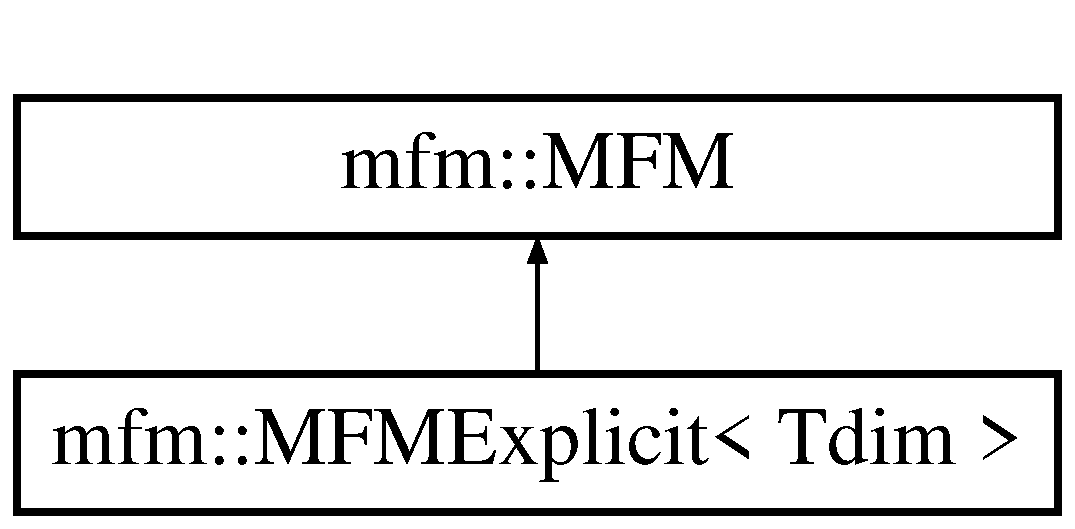
\includegraphics[height=2.000000cm]{classmfm_1_1_m_f_m}
\end{center}
\end{figure}
\subsection*{Public Member Functions}
\begin{DoxyCompactItemize}
\item 
\mbox{\Hypertarget{classmfm_1_1_m_f_m_acd16d85bab80502144c6743078a3ea33}\label{classmfm_1_1_m_f_m_acd16d85bab80502144c6743078a3ea33}} 
{\bfseries M\+FM} (std\+::unique\+\_\+ptr$<$ \hyperlink{classmfm_1_1_i_o}{IO} $>$ \&\&io)
\item 
\mbox{\Hypertarget{classmfm_1_1_m_f_m_a907d70cf1b581a589e1e6559cff52113}\label{classmfm_1_1_m_f_m_a907d70cf1b581a589e1e6559cff52113}} 
virtual bool {\bfseries initialise\+\_\+mesh} ()=0
\item 
\mbox{\Hypertarget{classmfm_1_1_m_f_m_aa5dcf9d73bcff53177a988911e30ec7d}\label{classmfm_1_1_m_f_m_aa5dcf9d73bcff53177a988911e30ec7d}} 
virtual bool {\bfseries initialise\+\_\+particles} ()=0
\item 
\mbox{\Hypertarget{classmfm_1_1_m_f_m_a26cb73bacc6dad74e87ef4ab0fef1c14}\label{classmfm_1_1_m_f_m_a26cb73bacc6dad74e87ef4ab0fef1c14}} 
virtual bool \hyperlink{classmfm_1_1_m_f_m_a26cb73bacc6dad74e87ef4ab0fef1c14}{initialise\+\_\+nodes} ()=0
\begin{DoxyCompactList}\small\item\em Intialise nodes. \end{DoxyCompactList}\item 
\mbox{\Hypertarget{classmfm_1_1_m_f_m_a0c824e2ab07dcdc96301a96df65090cd}\label{classmfm_1_1_m_f_m_a0c824e2ab07dcdc96301a96df65090cd}} 
virtual bool {\bfseries solve} ()=0
\end{DoxyCompactItemize}
\subsection*{Protected Attributes}
\begin{DoxyCompactItemize}
\item 
\mbox{\Hypertarget{classmfm_1_1_m_f_m_ae4a3f4844f4d9affcc9b814fbd89be96}\label{classmfm_1_1_m_f_m_ae4a3f4844f4d9affcc9b814fbd89be96}} 
std\+::string {\bfseries uuid\+\_\+}
\item 
\mbox{\Hypertarget{classmfm_1_1_m_f_m_a48087e7734feaeb0a8cf763a57a4f97b}\label{classmfm_1_1_m_f_m_a48087e7734feaeb0a8cf763a57a4f97b}} 
double \hyperlink{classmfm_1_1_m_f_m_a48087e7734feaeb0a8cf763a57a4f97b}{dt\+\_\+} \{std\+::numeric\+\_\+limits$<$double$>$\+::max()\}
\begin{DoxyCompactList}\small\item\em Time step size. \end{DoxyCompactList}\item 
\mbox{\Hypertarget{classmfm_1_1_m_f_m_a99a022cfd0a14d18a2b7e2449f35a8e1}\label{classmfm_1_1_m_f_m_a99a022cfd0a14d18a2b7e2449f35a8e1}} 
bool \hyperlink{classmfm_1_1_m_f_m_a99a022cfd0a14d18a2b7e2449f35a8e1}{axi\+\_\+} \{false\}
\begin{DoxyCompactList}\small\item\em A\+X\+I\+S\+Y\+M\+M\+E\+T\+R\+IC. \end{DoxyCompactList}\item 
\mbox{\Hypertarget{classmfm_1_1_m_f_m_a6b438e05bf767bda02514754c2ec6336}\label{classmfm_1_1_m_f_m_a6b438e05bf767bda02514754c2ec6336}} 
\hyperlink{namespacemfm_a7d021c8caa1852f673d78358edc6b7f9}{mfm\+::\+Index} \hyperlink{classmfm_1_1_m_f_m_a6b438e05bf767bda02514754c2ec6336}{step\+\_\+} \{0\}
\begin{DoxyCompactList}\small\item\em Current step. \end{DoxyCompactList}\item 
\mbox{\Hypertarget{classmfm_1_1_m_f_m_a5c9d196210bf508441ae90fbaf617954}\label{classmfm_1_1_m_f_m_a5c9d196210bf508441ae90fbaf617954}} 
\hyperlink{namespacemfm_a7d021c8caa1852f673d78358edc6b7f9}{mfm\+::\+Index} \hyperlink{classmfm_1_1_m_f_m_a5c9d196210bf508441ae90fbaf617954}{nsteps\+\_\+} \{std\+::numeric\+\_\+limits$<$\hyperlink{namespacemfm_a7d021c8caa1852f673d78358edc6b7f9}{mfm\+::\+Index}$>$\+::max()\}
\begin{DoxyCompactList}\small\item\em Number of steps. \end{DoxyCompactList}\item 
\mbox{\Hypertarget{classmfm_1_1_m_f_m_a797d222412df1eb7fcb68a1527d40574}\label{classmfm_1_1_m_f_m_a797d222412df1eb7fcb68a1527d40574}} 
std\+::unique\+\_\+ptr$<$ \hyperlink{classmfm_1_1_i_o}{mfm\+::\+IO} $>$ \hyperlink{classmfm_1_1_m_f_m_a797d222412df1eb7fcb68a1527d40574}{io\+\_\+}
\begin{DoxyCompactList}\small\item\em A unique ptr to \hyperlink{classmfm_1_1_i_o}{IO} object. \end{DoxyCompactList}\end{DoxyCompactItemize}


\subsection{Detailed Description}
\hyperlink{classmfm_1_1_m_f_m}{M\+FM} class  \hyperlink{classmfm_1_1_m_f_m}{M\+FM} class calls solver and algorithm  mfm class\+: implicit and explicit mfm 

The documentation for this class was generated from the following file\+:\begin{DoxyCompactItemize}
\item 
include/mfm.\+h\end{DoxyCompactItemize}

\hypertarget{classmfm_1_1_m_f_m_explicit}{}\section{mfm\+:\+:M\+F\+M\+Explicit$<$ Tdim $>$ Class Template Reference}
\label{classmfm_1_1_m_f_m_explicit}\index{mfm\+::\+M\+F\+M\+Explicit$<$ Tdim $>$@{mfm\+::\+M\+F\+M\+Explicit$<$ Tdim $>$}}


A class that implements the fully explicit mfm.  




{\ttfamily \#include $<$mfm\+\_\+explicit.\+h$>$}

Inheritance diagram for mfm\+:\+:M\+F\+M\+Explicit$<$ Tdim $>$\+:\begin{figure}[H]
\begin{center}
\leavevmode
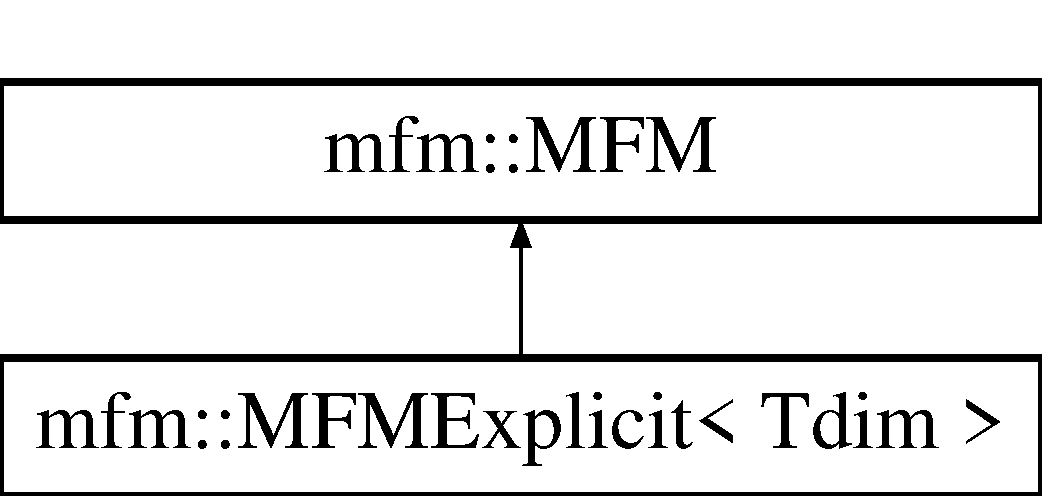
\includegraphics[height=2.000000cm]{classmfm_1_1_m_f_m_explicit}
\end{center}
\end{figure}
\subsection*{Public Member Functions}
\begin{DoxyCompactItemize}
\item 
\hyperlink{classmfm_1_1_m_f_m_explicit_a3b1473505cf73cd6c3589439d9216025}{M\+F\+M\+Explicit} (std\+::unique\+\_\+ptr$<$ \hyperlink{classmfm_1_1_i_o}{IO} $>$ \&\&io)
\begin{DoxyCompactList}\small\item\em Default constructor. \end{DoxyCompactList}\item 
\mbox{\Hypertarget{classmfm_1_1_m_f_m_explicit_a9621f2e63e9d3dd3e8f31c2fbe9e5b35}\label{classmfm_1_1_m_f_m_explicit_a9621f2e63e9d3dd3e8f31c2fbe9e5b35}} 
bool \hyperlink{classmfm_1_1_m_f_m_explicit_a9621f2e63e9d3dd3e8f31c2fbe9e5b35}{initialise\+\_\+mesh} () override
\begin{DoxyCompactList}\small\item\em Initialise mesh. \end{DoxyCompactList}\item 
\mbox{\Hypertarget{classmfm_1_1_m_f_m_explicit_a2067a261bf027b9c0a34cb94b0d55527}\label{classmfm_1_1_m_f_m_explicit_a2067a261bf027b9c0a34cb94b0d55527}} 
bool \hyperlink{classmfm_1_1_m_f_m_explicit_a2067a261bf027b9c0a34cb94b0d55527}{initialise\+\_\+nodes} () override
\begin{DoxyCompactList}\small\item\em Intialise nodes. \end{DoxyCompactList}\item 
\mbox{\Hypertarget{classmfm_1_1_m_f_m_explicit_a72d51d04855c10a843a654140f7f8c98}\label{classmfm_1_1_m_f_m_explicit_a72d51d04855c10a843a654140f7f8c98}} 
bool \hyperlink{classmfm_1_1_m_f_m_explicit_a72d51d04855c10a843a654140f7f8c98}{initialise\+\_\+particles} () override
\begin{DoxyCompactList}\small\item\em Initialise particles. \end{DoxyCompactList}\item 
\mbox{\Hypertarget{classmfm_1_1_m_f_m_explicit_a6d91f7c7dc52218f1a8aed74946c4391}\label{classmfm_1_1_m_f_m_explicit_a6d91f7c7dc52218f1a8aed74946c4391}} 
bool \hyperlink{classmfm_1_1_m_f_m_explicit_a6d91f7c7dc52218f1a8aed74946c4391}{solve} () override
\begin{DoxyCompactList}\small\item\em Solve. \end{DoxyCompactList}\end{DoxyCompactItemize}
\subsection*{Protected Attributes}
\begin{DoxyCompactItemize}
\item 
\mbox{\Hypertarget{classmfm_1_1_m_f_m_explicit_a8ffcb7f9541221c76a9ab163bb7d574e}\label{classmfm_1_1_m_f_m_explicit_a8ffcb7f9541221c76a9ab163bb7d574e}} 
std\+::unique\+\_\+ptr$<$ \hyperlink{classmfm_1_1_domain}{mfm\+::\+Domain}$<$ Tdim $>$ $>$ \hyperlink{classmfm_1_1_m_f_m_explicit_a8ffcb7f9541221c76a9ab163bb7d574e}{domain\+\_\+}
\begin{DoxyCompactList}\small\item\em \hyperlink{classmfm_1_1_domain}{Domain} object. \end{DoxyCompactList}\end{DoxyCompactItemize}


\subsection{Detailed Description}
\subsubsection*{template$<$unsigned Tdim$>$\newline
class mfm\+::\+M\+F\+M\+Explicit$<$ Tdim $>$}

A class that implements the fully explicit mfm. 

\hyperlink{classmfm_1_1_m_f_m_explicit}{M\+F\+M\+Explicit} class

A single-\/phase explicit M\+PM 
\begin{DoxyTemplParams}{Template Parameters}
{\em Tdim} & Dimension \\
\hline
\end{DoxyTemplParams}


\subsection{Constructor \& Destructor Documentation}
\mbox{\Hypertarget{classmfm_1_1_m_f_m_explicit_a3b1473505cf73cd6c3589439d9216025}\label{classmfm_1_1_m_f_m_explicit_a3b1473505cf73cd6c3589439d9216025}} 
\index{mfm\+::\+M\+F\+M\+Explicit@{mfm\+::\+M\+F\+M\+Explicit}!M\+F\+M\+Explicit@{M\+F\+M\+Explicit}}
\index{M\+F\+M\+Explicit@{M\+F\+M\+Explicit}!mfm\+::\+M\+F\+M\+Explicit@{mfm\+::\+M\+F\+M\+Explicit}}
\subsubsection{\texorpdfstring{M\+F\+M\+Explicit()}{MFMExplicit()}}
{\footnotesize\ttfamily template$<$unsigned Tdim$>$ \\
\hyperlink{classmfm_1_1_m_f_m_explicit}{mfm\+::\+M\+F\+M\+Explicit}$<$ Tdim $>$\+::\hyperlink{classmfm_1_1_m_f_m_explicit}{M\+F\+M\+Explicit} (\begin{DoxyParamCaption}\item[{std\+::unique\+\_\+ptr$<$ \hyperlink{classmfm_1_1_i_o}{IO} $>$ \&\&}]{io }\end{DoxyParamCaption})}



Default constructor. 

Constructor. 

The documentation for this class was generated from the following file\+:\begin{DoxyCompactItemize}
\item 
include/mfm\+\_\+explicit.\+h\end{DoxyCompactItemize}

\hypertarget{classmfm_1_1_node}{}\section{mfm\+:\+:Node$<$ Tdim $>$ Class Template Reference}
\label{classmfm_1_1_node}\index{mfm\+::\+Node$<$ Tdim $>$@{mfm\+::\+Node$<$ Tdim $>$}}
\subsection*{Public Types}
\begin{DoxyCompactItemize}
\item 
\mbox{\Hypertarget{classmfm_1_1_node_a528ae22876ff7f38409424f9db181727}\label{classmfm_1_1_node_a528ae22876ff7f38409424f9db181727}} 
using \hyperlink{classmfm_1_1_node_a528ae22876ff7f38409424f9db181727}{Vector\+Dim} = Eigen\+::\+Matrix$<$ double, Tdim, 1 $>$
\begin{DoxyCompactList}\small\item\em Define a vector of size dimension. \end{DoxyCompactList}\end{DoxyCompactItemize}
\subsection*{Public Member Functions}
\begin{DoxyCompactItemize}
\item 
\hyperlink{classmfm_1_1_node_ac5897f6e82a9d032cb22b14d5ac00ab9}{Node} (\hyperlink{namespacemfm_a7d021c8caa1852f673d78358edc6b7f9}{mfm\+::\+Index} id, const \hyperlink{classmfm_1_1_node_a528ae22876ff7f38409424f9db181727}{Vector\+Dim} \&coords)
\item 
\mbox{\Hypertarget{classmfm_1_1_node_acdfae40a74b72f3016b2f4f6fa9bfa56}\label{classmfm_1_1_node_acdfae40a74b72f3016b2f4f6fa9bfa56}} 
\hyperlink{classmfm_1_1_node_acdfae40a74b72f3016b2f4f6fa9bfa56}{$\sim$\+Node} ()
\begin{DoxyCompactList}\small\item\em Destructor. \end{DoxyCompactList}\item 
\mbox{\Hypertarget{classmfm_1_1_node_a5f37911f78ba13de4e3895b0acb6ac68}\label{classmfm_1_1_node_a5f37911f78ba13de4e3895b0acb6ac68}} 
\hyperlink{classmfm_1_1_node_a5f37911f78ba13de4e3895b0acb6ac68}{Node} (const \hyperlink{classmfm_1_1_node}{Node}$<$ Tdim $>$ \&)=delete
\begin{DoxyCompactList}\small\item\em Delete copy constructor. \end{DoxyCompactList}\item 
\mbox{\Hypertarget{classmfm_1_1_node_a61863270265a582ad503cadf99e515ee}\label{classmfm_1_1_node_a61863270265a582ad503cadf99e515ee}} 
\hyperlink{classmfm_1_1_node}{Node} \& \hyperlink{classmfm_1_1_node_a61863270265a582ad503cadf99e515ee}{operator=} (const \hyperlink{classmfm_1_1_node}{Node}$<$ Tdim $>$ \&)=delete
\begin{DoxyCompactList}\small\item\em Delete assignement operator. \end{DoxyCompactList}\item 
void \hyperlink{classmfm_1_1_node_a7744a3637ff17d5443ce965a73a571c2}{assign\+\_\+coordinates} (const \hyperlink{classmfm_1_1_node_a528ae22876ff7f38409424f9db181727}{Vector\+Dim} \&coord)
\end{DoxyCompactItemize}


\subsection{Constructor \& Destructor Documentation}
\mbox{\Hypertarget{classmfm_1_1_node_ac5897f6e82a9d032cb22b14d5ac00ab9}\label{classmfm_1_1_node_ac5897f6e82a9d032cb22b14d5ac00ab9}} 
\index{mfm\+::\+Node@{mfm\+::\+Node}!Node@{Node}}
\index{Node@{Node}!mfm\+::\+Node@{mfm\+::\+Node}}
\subsubsection{\texorpdfstring{Node()}{Node()}}
{\footnotesize\ttfamily template$<$unsigned Tdim$>$ \\
\hyperlink{classmfm_1_1_node}{mfm\+::\+Node}$<$ Tdim $>$\+::\hyperlink{classmfm_1_1_node}{Node} (\begin{DoxyParamCaption}\item[{\hyperlink{namespacemfm_a7d021c8caa1852f673d78358edc6b7f9}{mfm\+::\+Index}}]{id,  }\item[{const \hyperlink{classmfm_1_1_node_a528ae22876ff7f38409424f9db181727}{Vector\+Dim} \&}]{coords }\end{DoxyParamCaption})}

Constructor 
\begin{DoxyParams}{Parameters}
{\em } & \\
\hline
\end{DoxyParams}


\subsection{Member Function Documentation}
\mbox{\Hypertarget{classmfm_1_1_node_a7744a3637ff17d5443ce965a73a571c2}\label{classmfm_1_1_node_a7744a3637ff17d5443ce965a73a571c2}} 
\index{mfm\+::\+Node@{mfm\+::\+Node}!assign\+\_\+coordinates@{assign\+\_\+coordinates}}
\index{assign\+\_\+coordinates@{assign\+\_\+coordinates}!mfm\+::\+Node@{mfm\+::\+Node}}
\subsubsection{\texorpdfstring{assign\+\_\+coordinates()}{assign\_coordinates()}}
{\footnotesize\ttfamily template$<$unsigned Tdim$>$ \\
void \hyperlink{classmfm_1_1_node}{mfm\+::\+Node}$<$ Tdim $>$\+::assign\+\_\+coordinates (\begin{DoxyParamCaption}\item[{const \hyperlink{classmfm_1_1_node_a528ae22876ff7f38409424f9db181727}{Vector\+Dim} \&}]{coord }\end{DoxyParamCaption})\hspace{0.3cm}{\ttfamily [inline]}}

Assign coordaintes 
\begin{DoxyParams}[1]{Parameters}
\mbox{\tt in}  & {\em coord} & Assign coord as coordinates of the nodebase \\
\hline
\end{DoxyParams}


The documentation for this class was generated from the following file\+:\begin{DoxyCompactItemize}
\item 
include/node.\+h\end{DoxyCompactItemize}

\hypertarget{classmfm_1_1_particle}{}\section{mfm\+:\+:Particle$<$ dim $>$ Class Template Reference}
\label{classmfm_1_1_particle}\index{mfm\+::\+Particle$<$ dim $>$@{mfm\+::\+Particle$<$ dim $>$}}


Base class that stores the information about particles.  




{\ttfamily \#include $<$particle.\+h$>$}

Inheritance diagram for mfm\+:\+:Particle$<$ dim $>$\+:\begin{figure}[H]
\begin{center}
\leavevmode
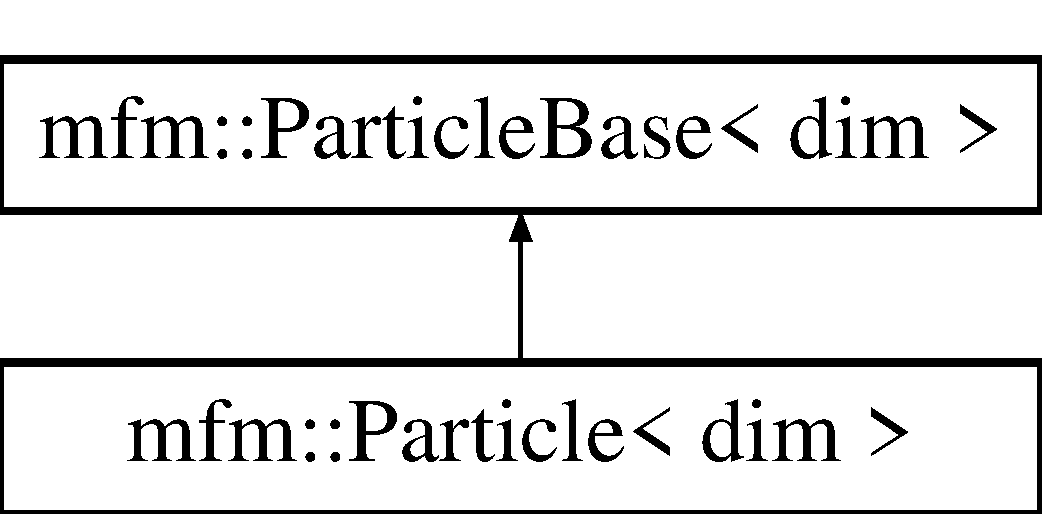
\includegraphics[height=2.000000cm]{classmfm_1_1_particle}
\end{center}
\end{figure}
\subsection*{Additional Inherited Members}


\subsection{Detailed Description}
\subsubsection*{template$<$unsigned dim$>$\newline
class mfm\+::\+Particle$<$ dim $>$}

Base class that stores the information about particles. 

\hyperlink{classmfm_1_1_particle}{Particle} class

\hyperlink{classmfm_1_1_particle}{Particle} class\+: id\+\_\+ and coordinates. 
\begin{DoxyTemplParams}{Template Parameters}
{\em Tdim} & Dimension \\
\hline
\end{DoxyTemplParams}


The documentation for this class was generated from the following file\+:\begin{DoxyCompactItemize}
\item 
include/particle.\+h\end{DoxyCompactItemize}

\hypertarget{classmfm_1_1_particle_base}{}\section{mfm\+:\+:Particle\+Base$<$ Tdim $>$ Class Template Reference}
\label{classmfm_1_1_particle_base}\index{mfm\+::\+Particle\+Base$<$ Tdim $>$@{mfm\+::\+Particle\+Base$<$ Tdim $>$}}


Base class that stores the information about particle\+Bases.  




{\ttfamily \#include $<$particle\+\_\+base.\+h$>$}

\subsection*{Public Types}
\begin{DoxyCompactItemize}
\item 
\mbox{\Hypertarget{classmfm_1_1_particle_base_afbf037646f60380710274aeddce74480}\label{classmfm_1_1_particle_base_afbf037646f60380710274aeddce74480}} 
using \hyperlink{classmfm_1_1_particle_base_afbf037646f60380710274aeddce74480}{Vector\+Dim} = Eigen\+::\+Matrix$<$ double, Tdim, 1 $>$
\begin{DoxyCompactList}\small\item\em Define a vector of size dimension. \end{DoxyCompactList}\end{DoxyCompactItemize}
\subsection*{Public Member Functions}
\begin{DoxyCompactItemize}
\item 
\hyperlink{classmfm_1_1_particle_base_a7e54d8eed2348cf828c643bdd4fe64fe}{Particle\+Base} (\hyperlink{namespacemfm_a7d021c8caa1852f673d78358edc6b7f9}{Index} \hyperlink{classmfm_1_1_particle_base_af0e7293eaedd690be27619c9add4066c}{id}, const \hyperlink{classmfm_1_1_particle_base_afbf037646f60380710274aeddce74480}{Vector\+Dim} \&coord)
\item 
\mbox{\Hypertarget{classmfm_1_1_particle_base_ac833dd416abf6158b45b54355f8c60f9}\label{classmfm_1_1_particle_base_ac833dd416abf6158b45b54355f8c60f9}} 
virtual \hyperlink{classmfm_1_1_particle_base_ac833dd416abf6158b45b54355f8c60f9}{$\sim$\+Particle\+Base} ()
\begin{DoxyCompactList}\small\item\em Destructor. \end{DoxyCompactList}\item 
\mbox{\Hypertarget{classmfm_1_1_particle_base_af0e7293eaedd690be27619c9add4066c}\label{classmfm_1_1_particle_base_af0e7293eaedd690be27619c9add4066c}} 
\hyperlink{namespacemfm_a7d021c8caa1852f673d78358edc6b7f9}{Index} \hyperlink{classmfm_1_1_particle_base_af0e7293eaedd690be27619c9add4066c}{id} () const
\begin{DoxyCompactList}\small\item\em Return id of the particle\+Base. \end{DoxyCompactList}\item 
void \hyperlink{classmfm_1_1_particle_base_a8ba22c9e8a5f67995013241843a3c0f4}{assign\+\_\+coordinates} (const \hyperlink{classmfm_1_1_particle_base_afbf037646f60380710274aeddce74480}{Vector\+Dim} \&coord)
\end{DoxyCompactItemize}
\subsection*{Protected Attributes}
\begin{DoxyCompactItemize}
\item 
\mbox{\Hypertarget{classmfm_1_1_particle_base_a8615262fcefb458f6c54e961f7758dc7}\label{classmfm_1_1_particle_base_a8615262fcefb458f6c54e961f7758dc7}} 
\hyperlink{classmfm_1_1_particle_base_afbf037646f60380710274aeddce74480}{Vector\+Dim} \hyperlink{classmfm_1_1_particle_base_a8615262fcefb458f6c54e961f7758dc7}{coordinates\+\_\+}
\begin{DoxyCompactList}\small\item\em coordinates \end{DoxyCompactList}\item 
\mbox{\Hypertarget{classmfm_1_1_particle_base_ac8d0e6602af1a9381e478d035c4f6a13}\label{classmfm_1_1_particle_base_ac8d0e6602af1a9381e478d035c4f6a13}} 
\hyperlink{namespacemfm_a7d021c8caa1852f673d78358edc6b7f9}{Index} \hyperlink{classmfm_1_1_particle_base_ac8d0e6602af1a9381e478d035c4f6a13}{id\+\_\+}
\begin{DoxyCompactList}\small\item\em particle\+Base iD \end{DoxyCompactList}\item 
\mbox{\Hypertarget{classmfm_1_1_particle_base_ae6f5538c34fcb799a00440b443001f6d}\label{classmfm_1_1_particle_base_ae6f5538c34fcb799a00440b443001f6d}} 
int \hyperlink{classmfm_1_1_particle_base_ae6f5538c34fcb799a00440b443001f6d}{cell\+\_\+id}
\begin{DoxyCompactList}\small\item\em Cell id. \end{DoxyCompactList}\item 
\mbox{\Hypertarget{classmfm_1_1_particle_base_ae9827d1ff93998e4f0d64936ccb8d1d8}\label{classmfm_1_1_particle_base_ae9827d1ff93998e4f0d64936ccb8d1d8}} 
Eigen\+::\+Matrix$<$ double, Tdim, 1 $>$ \hyperlink{classmfm_1_1_particle_base_ae9827d1ff93998e4f0d64936ccb8d1d8}{xi\+\_\+}
\begin{DoxyCompactList}\small\item\em Reference coordinates (in a cell) \end{DoxyCompactList}\end{DoxyCompactItemize}


\subsection{Detailed Description}
\subsubsection*{template$<$unsigned Tdim$>$\newline
class mfm\+::\+Particle\+Base$<$ Tdim $>$}

Base class that stores the information about particle\+Bases. 

\hyperlink{classmfm_1_1_particle_base}{Particle\+Base} class

\hyperlink{classmfm_1_1_particle_base}{Particle\+Base} class\+: id\+\_\+ and coordinates. 
\begin{DoxyTemplParams}{Template Parameters}
{\em Tdim} & Dimension \\
\hline
\end{DoxyTemplParams}


\subsection{Constructor \& Destructor Documentation}
\mbox{\Hypertarget{classmfm_1_1_particle_base_a7e54d8eed2348cf828c643bdd4fe64fe}\label{classmfm_1_1_particle_base_a7e54d8eed2348cf828c643bdd4fe64fe}} 
\index{mfm\+::\+Particle\+Base@{mfm\+::\+Particle\+Base}!Particle\+Base@{Particle\+Base}}
\index{Particle\+Base@{Particle\+Base}!mfm\+::\+Particle\+Base@{mfm\+::\+Particle\+Base}}
\subsubsection{\texorpdfstring{Particle\+Base()}{ParticleBase()}}
{\footnotesize\ttfamily template$<$unsigned Tdim$>$ \\
\hyperlink{classmfm_1_1_particle_base}{mfm\+::\+Particle\+Base}$<$ Tdim $>$\+::\hyperlink{classmfm_1_1_particle_base}{Particle\+Base} (\begin{DoxyParamCaption}\item[{\hyperlink{namespacemfm_a7d021c8caa1852f673d78358edc6b7f9}{Index}}]{id,  }\item[{const \hyperlink{classmfm_1_1_particle_base_afbf037646f60380710274aeddce74480}{Vector\+Dim} \&}]{coord }\end{DoxyParamCaption})}

Constructor with id and coordinates 
\begin{DoxyParams}[1]{Parameters}
\mbox{\tt in}  & {\em id} & \hyperlink{classmfm_1_1_particle}{Particle} id \\
\hline
\mbox{\tt in}  & {\em coord} & coordinates of the particle \\
\hline
\end{DoxyParams}


\subsection{Member Function Documentation}
\mbox{\Hypertarget{classmfm_1_1_particle_base_a8ba22c9e8a5f67995013241843a3c0f4}\label{classmfm_1_1_particle_base_a8ba22c9e8a5f67995013241843a3c0f4}} 
\index{mfm\+::\+Particle\+Base@{mfm\+::\+Particle\+Base}!assign\+\_\+coordinates@{assign\+\_\+coordinates}}
\index{assign\+\_\+coordinates@{assign\+\_\+coordinates}!mfm\+::\+Particle\+Base@{mfm\+::\+Particle\+Base}}
\subsubsection{\texorpdfstring{assign\+\_\+coordinates()}{assign\_coordinates()}}
{\footnotesize\ttfamily template$<$unsigned Tdim$>$ \\
void \hyperlink{classmfm_1_1_particle_base}{mfm\+::\+Particle\+Base}$<$ Tdim $>$\+::assign\+\_\+coordinates (\begin{DoxyParamCaption}\item[{const \hyperlink{classmfm_1_1_particle_base_afbf037646f60380710274aeddce74480}{Vector\+Dim} \&}]{coord }\end{DoxyParamCaption})\hspace{0.3cm}{\ttfamily [inline]}}

Assign coordinates 
\begin{DoxyParams}[1]{Parameters}
\mbox{\tt in}  & {\em coord} & Assign coord as coordinates of the particle\+Base \\
\hline
\end{DoxyParams}


The documentation for this class was generated from the following file\+:\begin{DoxyCompactItemize}
\item 
include/particle\+\_\+base.\+h\end{DoxyCompactItemize}

\hypertarget{classmfm_1_1_quadrature}{}\section{mfm\+:\+:Quadrature$<$ dim $>$ Class Template Reference}
\label{classmfm_1_1_quadrature}\index{mfm\+::\+Quadrature$<$ dim $>$@{mfm\+::\+Quadrature$<$ dim $>$}}


The documentation for this class was generated from the following file\+:\begin{DoxyCompactItemize}
\item 
include/quadrature.\+h\end{DoxyCompactItemize}

\hypertarget{classmfm_1_1_read_mesh}{}\section{mfm\+:\+:Read\+Mesh$<$ Tdim $>$ Class Template Reference}
\label{classmfm_1_1_read_mesh}\index{mfm\+::\+Read\+Mesh$<$ Tdim $>$@{mfm\+::\+Read\+Mesh$<$ Tdim $>$}}


Class that returns mesh and particles locataions based on G\+Mesh ascii file.  




{\ttfamily \#include $<$read\+\_\+mesh.\+h$>$}

\subsection*{Public Types}
\begin{DoxyCompactItemize}
\item 
\mbox{\Hypertarget{classmfm_1_1_read_mesh_a0dcd4f554ae2784be3fa53e547b2f6a9}\label{classmfm_1_1_read_mesh_a0dcd4f554ae2784be3fa53e547b2f6a9}} 
using \hyperlink{classmfm_1_1_read_mesh_a0dcd4f554ae2784be3fa53e547b2f6a9}{Vector\+Dim} = Eigen\+::\+Matrix$<$ double, Tdim, 1 $>$
\begin{DoxyCompactList}\small\item\em Define a vector of size dimension. \end{DoxyCompactList}\end{DoxyCompactItemize}
\subsection*{Public Member Functions}
\begin{DoxyCompactItemize}
\item 
\mbox{\Hypertarget{classmfm_1_1_read_mesh_aca466723f1ea120fc76ec8cee2e62a98}\label{classmfm_1_1_read_mesh_aca466723f1ea120fc76ec8cee2e62a98}} 
\hyperlink{classmfm_1_1_read_mesh_aca466723f1ea120fc76ec8cee2e62a98}{Read\+Mesh} ()
\begin{DoxyCompactList}\small\item\em Constructor. \end{DoxyCompactList}\item 
\hyperlink{classmfm_1_1_read_mesh_a205f0231970ab4511eb07ba7ecfcff47}{Read\+Mesh} (std\+::string filename)
\item 
std\+::vector$<$ std\+::vector$<$ \hyperlink{namespacemfm_a7d021c8caa1852f673d78358edc6b7f9}{mfm\+::\+Index} $>$ $>$ \hyperlink{classmfm_1_1_read_mesh_a7fe80e6e5bec7a835ffa03ef5ad92056}{read\+\_\+mesh\+\_\+cells} (const std\+::string \&mesh)
\item 
std\+::vector$<$ \hyperlink{classmfm_1_1_read_mesh_a0dcd4f554ae2784be3fa53e547b2f6a9}{Vector\+Dim} $>$ \hyperlink{classmfm_1_1_read_mesh_aad9a82f738f2f49010a5ca7c218855ce}{read\+\_\+nodes} ()
\end{DoxyCompactItemize}


\subsection{Detailed Description}
\subsubsection*{template$<$unsigned Tdim$>$\newline
class mfm\+::\+Read\+Mesh$<$ Tdim $>$}

Class that returns mesh and particles locataions based on G\+Mesh ascii file. 

\hyperlink{classmfm_1_1_read_mesh}{Read\+Mesh} class 
\begin{DoxyTemplParams}{Template Parameters}
{\em Tdim} & Dimension \\
\hline
\end{DoxyTemplParams}


\subsection{Constructor \& Destructor Documentation}
\mbox{\Hypertarget{classmfm_1_1_read_mesh_a205f0231970ab4511eb07ba7ecfcff47}\label{classmfm_1_1_read_mesh_a205f0231970ab4511eb07ba7ecfcff47}} 
\index{mfm\+::\+Read\+Mesh@{mfm\+::\+Read\+Mesh}!Read\+Mesh@{Read\+Mesh}}
\index{Read\+Mesh@{Read\+Mesh}!mfm\+::\+Read\+Mesh@{mfm\+::\+Read\+Mesh}}
\subsubsection{\texorpdfstring{Read\+Mesh()}{ReadMesh()}}
{\footnotesize\ttfamily template$<$unsigned Tdim$>$ \\
\hyperlink{classmfm_1_1_read_mesh}{mfm\+::\+Read\+Mesh}$<$ Tdim $>$\+::\hyperlink{classmfm_1_1_read_mesh}{Read\+Mesh} (\begin{DoxyParamCaption}\item[{std\+::string}]{filename }\end{DoxyParamCaption})\hspace{0.3cm}{\ttfamily [inline]}}

Constructor with filename 
\begin{DoxyParams}[1]{Parameters}
\mbox{\tt in}  & {\em filename} & with name of file \\
\hline
\end{DoxyParams}
filename\+\_\+ 

\subsection{Member Function Documentation}
\mbox{\Hypertarget{classmfm_1_1_read_mesh_a7fe80e6e5bec7a835ffa03ef5ad92056}\label{classmfm_1_1_read_mesh_a7fe80e6e5bec7a835ffa03ef5ad92056}} 
\index{mfm\+::\+Read\+Mesh@{mfm\+::\+Read\+Mesh}!read\+\_\+mesh\+\_\+cells@{read\+\_\+mesh\+\_\+cells}}
\index{read\+\_\+mesh\+\_\+cells@{read\+\_\+mesh\+\_\+cells}!mfm\+::\+Read\+Mesh@{mfm\+::\+Read\+Mesh}}
\subsubsection{\texorpdfstring{read\+\_\+mesh\+\_\+cells()}{read\_mesh\_cells()}}
{\footnotesize\ttfamily template$<$unsigned Tdim$>$ \\
std\+::vector$<$std\+::vector$<$\hyperlink{namespacemfm_a7d021c8caa1852f673d78358edc6b7f9}{mfm\+::\+Index}$>$ $>$ \hyperlink{classmfm_1_1_read_mesh}{mfm\+::\+Read\+Mesh}$<$ Tdim $>$\+::read\+\_\+mesh\+\_\+cells (\begin{DoxyParamCaption}\item[{const std\+::string \&}]{mesh }\end{DoxyParamCaption})}

Read mesh cells file 
\begin{DoxyParams}[1]{Parameters}
\mbox{\tt in}  & {\em mesh} & file name with nodes and cells \\
\hline
\end{DoxyParams}

\begin{DoxyRetVals}{Return values}
{\em cells} & Vector of nodal indices of cells \\
\hline
\end{DoxyRetVals}
\mbox{\Hypertarget{classmfm_1_1_read_mesh_aad9a82f738f2f49010a5ca7c218855ce}\label{classmfm_1_1_read_mesh_aad9a82f738f2f49010a5ca7c218855ce}} 
\index{mfm\+::\+Read\+Mesh@{mfm\+::\+Read\+Mesh}!read\+\_\+nodes@{read\+\_\+nodes}}
\index{read\+\_\+nodes@{read\+\_\+nodes}!mfm\+::\+Read\+Mesh@{mfm\+::\+Read\+Mesh}}
\subsubsection{\texorpdfstring{read\+\_\+nodes()}{read\_nodes()}}
{\footnotesize\ttfamily template$<$unsigned Tdim$>$ \\
std\+::vector$<$ Eigen\+::\+Matrix$<$ double, Tdim, 1 $>$ $>$ \hyperlink{classmfm_1_1_read_mesh}{mfm\+::\+Read\+Mesh}$<$ Tdim $>$\+::read\+\_\+nodes (\begin{DoxyParamCaption}{ }\end{DoxyParamCaption})}

Read particles file 
\begin{DoxyParams}[1]{Parameters}
\mbox{\tt in}  & {\em particles\+\_\+files} & file name with particle coordinates \\
\hline
\end{DoxyParams}

\begin{DoxyRetVals}{Return values}
{\em coordinates} & Vector of particle coordinates \\
\hline
\end{DoxyRetVals}


The documentation for this class was generated from the following file\+:\begin{DoxyCompactItemize}
\item 
include/read\+\_\+mesh.\+h\end{DoxyCompactItemize}

%--- End generated contents ---

% Index
\backmatter
\newpage
\phantomsection
\clearemptydoublepage
\addcontentsline{toc}{chapter}{Index}
\printindex

\end{document}
